\documentclass[aspectratio=169]{beamer}
\usepackage[utf8]{inputenc}

\usepackage{listings}

\lstset{
    basicstyle=\linespread{1}\scriptsize\ttfamily, 
    numbers=left,
    stepnumber=1,
    showstringspaces=false,
    columns=fullflexible,
    tabsize=2,
    frame=single,
    breakatwhitespace=true,  
    breaklines=true,
    captionpos=b, 
    numberstyle=\tiny,
}

\usetheme{default}
\usecolortheme{seahorse}
\setbeamertemplate{navigation symbols}{}

\AtBeginSection[]
{
    \begin{frame}
        \frametitle{Table of Contents}
        \tableofcontents[currentsection]
    \end{frame}
}

\setbeamertemplate{section in toc}[sections numbered]
\setbeamertemplate{subsection in toc}[subsections numbered]

\title{Intorduction to Python}
\subtitle{Scientific Computing}
\author{Stefan Abi-Karam}
\date{Summer 2023}


\begin{document}

\begin{frame}
    \titlepage
\end{frame}

\begin{frame}{Table of Contents}
    \tableofcontents
\end{frame}

\section{Pyhton Overview}

\begin{frame}{What Is Python}
    \begin{columns}
        \begin{column}{0.3\textwidth}
            \centering
            
\includegraphics[width=\textwidth]{imgs/python_logo.png}
        \end{column}
        \begin{column}{0.7\textwidth}
            \begin{itemize}
                \item Python is an interpreted, high-level, general-purpose programming language
                \item Interpreted means there is no python-to-assembly compiler, someone wrote and compiled a program in C (CPython) which is a program that just reads and executes your Python code
                \item Python also has a large standard library to achieve most tasks with relatively little code
                \item There are thousands of other libraries out that that other people have written that you can download and import into your code to do more complex stuff (ex. scientific computations and plotting)
            \end{itemize}
        \end{column}
    \end{columns}
\end{frame}

\begin{frame}{Compiled Program vs. Interpreted Program}
    \centering
    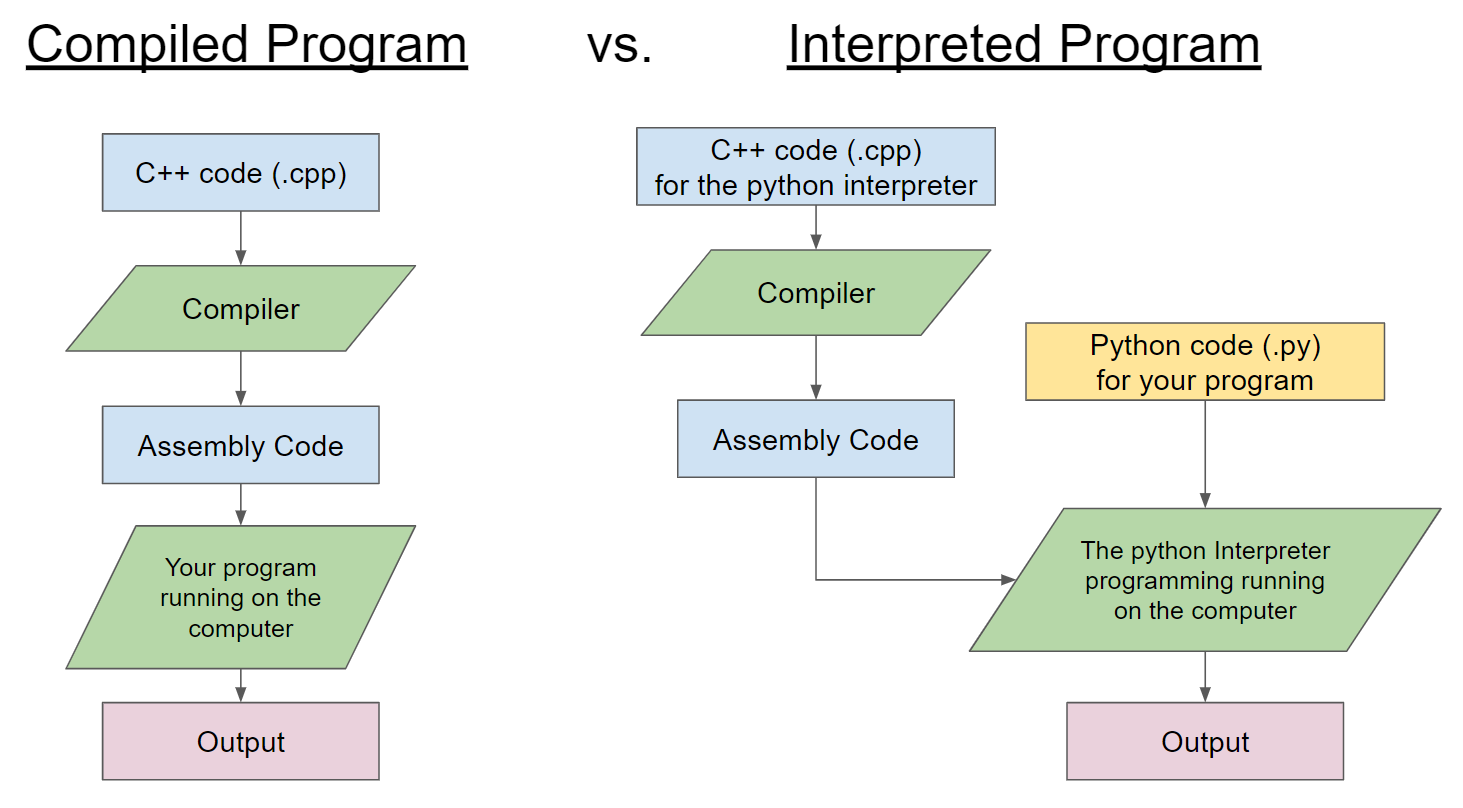
\includegraphics[width=\textwidth]{imgs/compiled_v_interpreted.png}
\end{frame}

\begin{frame}{Why Choose Python}
    % - Least amount of friction from the idea in your head you want to answer research question about to executing code that works and answers those questions
    % - Python has a large community across many different fields of research
    %     - Very strong popularity in scientific computing and data science
    % This means that many people in these fields has put in effort to write and maintain python libraries specific for scientific computing and data science
    % - If there is no libraries for a specific task you are trying to do or area you are woking in you can easily package your code and publish it as its own library for other to use
    \begin{itemize}
        \item There is the least amount of friction from the idea in your head to executing code that works and answers your research questions
        \item Python has a large community across many different fields of research
              \begin{itemize}
                  \item Very strong popularity in scientific computing and data science
              \end{itemize}
        \item This means that many people in these fields has put in effort to write and maintain python libraries specific for scientific computing and data science
        \item In the absence of libraries for a particular task you are attempting or area of expertise you are working in, you can easily package and publish your code as its own library.
    \end{itemize}
\end{frame}

\begin{frame}{Why Choose Python}
    \centering
    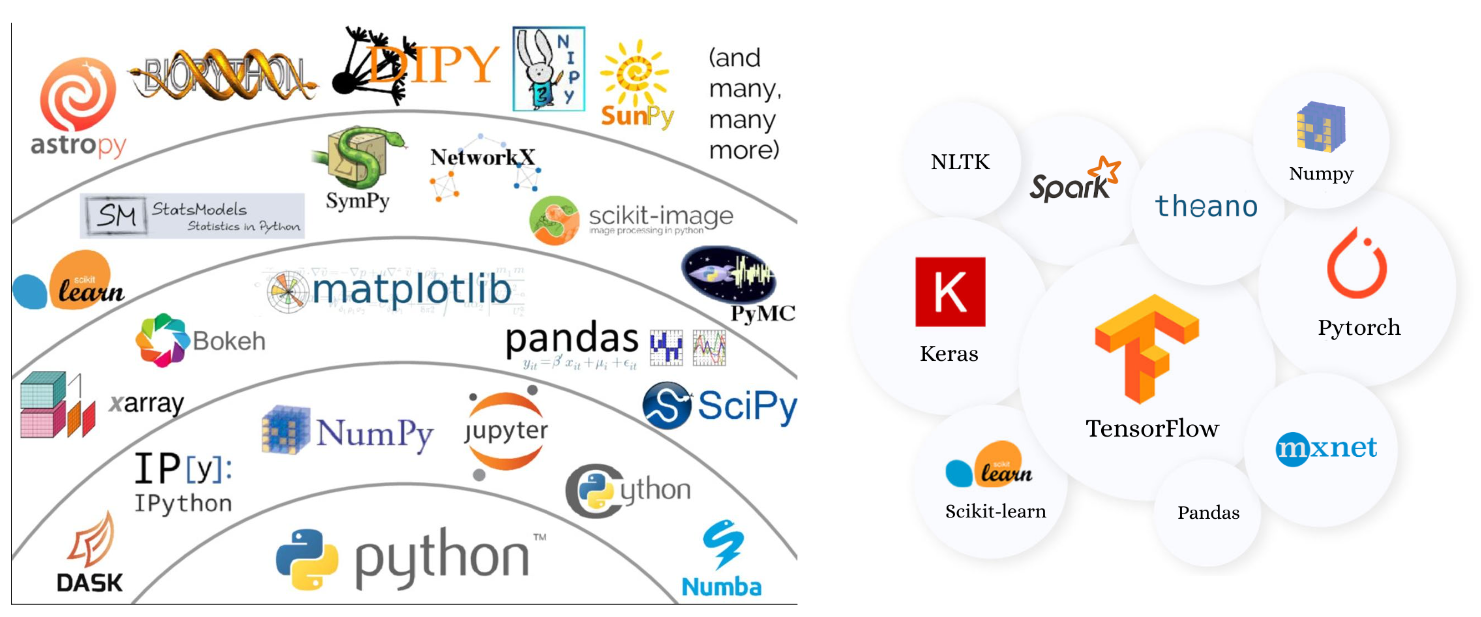
\includegraphics[width=\textwidth]{imgs/python_packages_examples.png}
\end{frame}

\section{Installation and Usage}

\begin{frame}{Python Installation and Versions}
    \begin{itemize}
        \item When you install Python you download a version of the Python interpreter
        \item Please use version 3.9, it has the newest features and supported by most libraries you will use
        \item You can install multiple versions on the same computer, you just end up with more than one interpreter you can use
        \item If you want to download Python you can do so at their website: \url{https://www.python.org/}
        \item There's also a program called Conda / Anaconda that used a lot in the research community to manage Python installations and other libraries you may want to install and use
        \item \textbf{I recommend using Conda to install Python and manage your Python environment and packages if you are going to install Python on your own computer}
    \end{itemize}
\end{frame}

\begin{frame}[fragile]{Using Python}
    Once Python is installed on your machine you can you use the Python command to run programs in the command line
    \begin{lstlisting}
> python your_file.py
    \end{lstlisting}

    \vspace{\baselineskip}

    Each Python installation also comes with a package manager named \texttt{pip} which you can also run from command line
    \begin{lstlisting}
> pip install numpy
    \end{lstlisting}

    \vspace{\baselineskip}

    If you are using Conda, you can call the \texttt{conda} command to install packages and manage Conda environments
    \begin{lstlisting}
> conda install numpy
    \end{lstlisting}
\end{frame}


\section{Python Core Concepts}

\subsection{Types}

\begin{frame}{What Are Types}

    \begin{itemize}
        \item Types are a way to classify objects
        \item Each object has a type
        \item Types are used to define how you can use the object
    \end{itemize}

\end{frame}


\begin{frame}{Python Types}

    \begin{columns}
        \begin{column}{0.5\textwidth}
            \begin{itemize}
                \item Numeric Types
                      \begin{itemize}
                          \item \texttt{int}: Integer Number
                          \item \texttt{float}: Floating Point Number (decimal)
                          \item \texttt{complex}: Complex Number
                      \end{itemize}
                \item Sequence Types
                      \begin{itemize}
                          \item \texttt{list}: List (mutable)
                          \item \texttt{tuple}: Like List (immutable)
                          \item \texttt{range}: Immutable sequence of numbers
                      \end{itemize}

                \item Text and Binary Sequence Types
                      \begin{itemize}
                          \item \texttt{str}: String (text / immutable sequence of characters)                          \item \texttt{bytes}: Immutable array of bytes
                          \item \texttt{bytes}: Immutable array of bytes
                      \end{itemize}
            \end{itemize}

        \end{column}
        \begin{column}{0.5\textwidth}
            \begin{itemize}

                \item Set Types
                      \begin{itemize}
                          \item \texttt{set}: Set (same usage as mathematical set)
                      \end{itemize}

                \item Mapping Types
                      \begin{itemize}
                          \item \texttt{dict}: Dictionary (new concept to most of you)

                      \end{itemize}
                \item Other Types
                      \begin{itemize}
                          \item \texttt{function}: function object
                          \item \texttt{module}: collection of functions, variables, and other objects
                          \item \texttt{bool}: Boolean Values (\texttt{True} / \texttt{False})
                          \item \texttt{None}: Null object (with value ``None'')
                      \end{itemize}
            \end{itemize}
        \end{column}
    \end{columns}
\end{frame}

\begin{frame}{Python Type Tree}
    \centering
    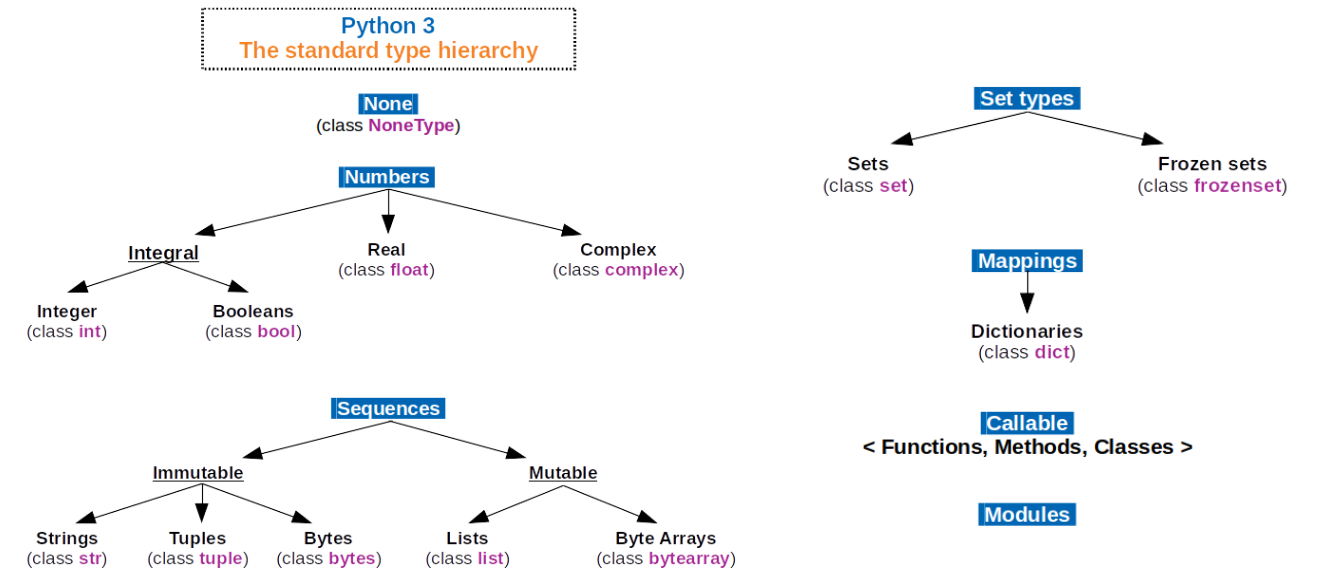
\includegraphics[width=\textwidth]{imgs/type_tree.png}
\end{frame}

\begin{frame}{Benefits of Types}
    \begin{itemize}
        \item \textbf{Operations}: Some operations between objects require the objects to be the same type
        \item \textbf{Comparisons}: Types allow for you to define how you can compare objects of different or same types
        \item \textbf{Builtin Functions}: Different types have different built in functions that let you things that make sense only with that type
        \item \textbf{Conversion Methods}: Each type may also have defined how to convert it to another type
    \end{itemize}
\end{frame}

\begin{frame}{Types in Programming Languages}
    \centering
    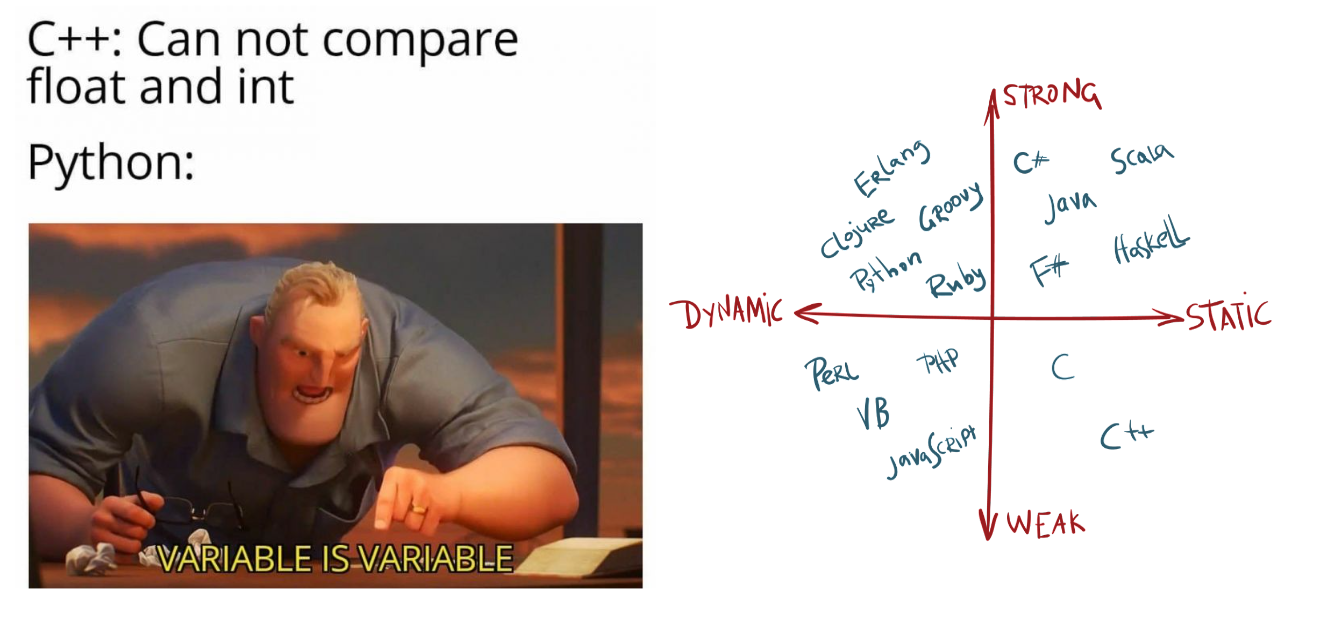
\includegraphics[width=\textwidth]{imgs/types_meme.png}
\end{frame}

\subsection{Variables}

\begin{frame}
    \frametitle{Python Variables}

    \begin{itemize}
        \item Variables are used to store values in a program.
        \item In Python, variables are created when you assign a value to them.
        \item Variables can be of \textbf{any type}, such as integers, floats, strings, and booleans.
    \end{itemize}

\end{frame}

\begin{frame}[fragile]
    \frametitle{Python Variables Examples}

    \begin{lstlisting}[language=Python,caption={Simple Variable Assignment}]
x = 5
y = 10
z = x + y
print(z) # this will print 15
    \end{lstlisting}
    \begin{lstlisting}[language=Python, caption={Reassigning Variables}]
x = 5
print(x) # this will print 5
x = "Hello"
print(x) # this will print "Hello"
    \end{lstlisting}
\end{frame}

\subsection{Operators and Expressions}

\begin{frame}{Operators}
    \begin{itemize}
        \item Operators are used to perform operations on variables and values.
        \item Python divides the operators in the following groups:
              \begin{itemize}
                  \item Arithmetic operators
                  \item Assignment operators
                  \item Comparison operators
                  \item Logical operators
                  \item Identity operators
                  \item Membership operators
                  \item Bitwise operators
              \end{itemize}
    \end{itemize}
\end{frame}

\begin{frame}{Arithmetic Operators}
    Arithmetic operators are used with numeric values to perform common mathematical operations:
    \begin{itemize}
        \item \texttt{x + y}: Addition
        \item \texttt{x - y}: Subtraction
        \item \texttt{x * y}: Multiplication
        \item \texttt{x / y}: Division
        \item \texttt{x \% y}: Modulus, remainder of x divided by y, only works with integers
        \item \texttt{x ** y}: Exponentiation, x to the power of y
        \item \texttt{x // y}: Floor Division, x divided by y rounded down to the nearest integer
    \end{itemize}
\end{frame}

\begin{frame}{Assignment Operators}
    Assignment operators are used to both compute and assign values to variables:
    \begin{itemize}
        \item \texttt{x = y}: Assignment, store the value of y in x
        \item \texttt{x += y}: Addition, add y to x and store the result in x
        \item \texttt{x -= y}: Subtraction, subtract y from x and store the result in x
        \item \texttt{x *= y}: Multiplication, multiply x by y and store the result in x
        \item \texttt{x /= y}: Division, divide x by y and store the result in x
        \item \texttt{x \%= y}: Modulus, divide x by y and store the remainder in x
        \item \texttt{x **= y}: Exponentiation, raise x to the power of y and store the result in x
        \item \texttt{x //= y}: Floor Division, divide x by y, round down to the nearest integer, and store the result in x
    \end{itemize}
\end{frame}

\begin{frame}{Comparison Operators}

    Comparison operators are used to compare two values:
    \begin{itemize}
        \item \texttt{x == y}: Equality
        \item \texttt{x != y}: Inequality
        \item \texttt{x > y}: Greater than
        \item \texttt{x < y}: Less than
        \item \texttt{x >= y}: Greater than or equal to
        \item \texttt{x <= y}: Less than or equal to
    \end{itemize}
\end{frame}

\begin{frame}{Logical Operators}
    Logical operators are used to combine conditional statements:
    \begin{itemize}
        \item \texttt{x and y}: AND operator; if both statements are true, the result is true
        \item \texttt{x or y}: OR operator; if one of the statements is true, the result is true
        \item \texttt{not x}: NOT operator; returns the opposite of the value
    \end{itemize}
\end{frame}

\begin{frame}{Identity Operators}
    Identity operators are used to compare the objects, not if they are equal, but if they are actually the same object, with the same memory location:
    \begin{itemize}
        \item \texttt{x is y}: Returns true if both variables are the same object instance
        \item \texttt{x is not y}: Returns true if both variables are not the same object instance
    \end{itemize}
\end{frame}

\begin{frame}{Membership Operators}
    Membership operators are used to test if a sequence is presented in an object:
    \begin{itemize}
        \item \texttt{x in y}: Check if object x is in sequence y
        \item \texttt{x not in y}: Check if object x is not in sequence y
    \end{itemize}
\end{frame}

\begin{frame}{Bitwise Operators}
    Bitwise operators are used to compare binary values:
    \begin{itemize}
        \item \texttt{x << y}: Shift bits in x to the left by y places, same as \texttt{x * (2 ** y)}
        \item \texttt{x >> y}: Shift bits in x to the right by y places, same as \texttt{x / (2 ** y)}
        \item \texttt{x \& y}: Bitwise AND
        \item \texttt{x | y}: Bitwise OR
        \item \texttt{$\sim$ x}: Bitwise NOT
        \item \texttt{x \string^ y}: Bitwise XOR, if both bits are the same, the result is 0, otherwise the result is 1.
    \end{itemize}
\end{frame}


\subsection{Control Flow}

\begin{frame}{Control Flow}
    \begin{itemize}
        \item Control flow statements are used to change the execution order of the program.
        \item Python supports the following control flow statements:
              \begin{itemize}
                  \item \texttt{if} statement
                  \item \texttt{else} statement
                  \item \texttt{elif} statement
              \end{itemize}
    \end{itemize}
\end{frame}

% example code with if statement
\begin{frame}[fragile]
    \frametitle{If Example}
    \begin{lstlisting}[language=Python, caption={If Statement}]
x = 5
y = 10
if x > y:
    print("x is greater than y")
    \end{lstlisting}

    \begin{itemize}
        \item What will happen when we run this code?
        \item What will happen when we change the value of x to 10?
    \end{itemize}
\end{frame}

% example code with if else statement
\begin{frame}[fragile]
    \frametitle{If-Else Example}
    \begin{lstlisting}[language=Python, caption={If-Else Statement}]
x = 5
y = 10
if x > y:
    print("x is greater than y")
else:
    print("x is less than or equal to y")
    \end{lstlisting}

    \begin{itemize}
        \item What will happen when we run this code?
        \item What will happen when we change the value of x to 10?
    \end{itemize}
\end{frame}

% example code with if elif else statement
\begin{frame}[fragile]
    \frametitle{If-Elif-Else Example}
    \begin{lstlisting}[language=Python, caption={If-Elif-Else Statement}]
x = 5
y = 10
if x > y:
    print("x is greater than y")
elif x == y:
    print("x is equal to y")
elif x < y:
    print("x is less than y")
else:
    print("How did we get here?")
\end{lstlisting}

    \begin{itemize}
        \item What will happen when we run this code?
        \item What will happen when we change the value of x to 10?
        \item What will happen when we change the value of x to 15?
        \item Can this code ever reach the \texttt{else} statement?
        \item What will happen when we change the value of x to "hello"?
    \end{itemize}
\end{frame}

\subsection{Loops}

\begin{frame}{Loops}
    \begin{itemize}
        \item Loops are used to repeat a block of code.
        \item Python supports common patterns of loops:
              \begin{itemize}
                  \item \texttt{while} loop
                  \item \texttt{for} loop
              \end{itemize}
    \end{itemize}
\end{frame}

% example code with while loop
\begin{frame}[fragile]
    \frametitle{While Loop Example}
    \begin{lstlisting}[language=Python, caption={Simple While Loop}]
x = 0
while x < 5:
    print(x)
    x += 1
\end{lstlisting}

    \begin{itemize}
        \item What will happen when we run this code?
        \item What will happen if we change the value of x to 2?
        \item What will happen if we change the value of x to 10?
    \end{itemize}
\end{frame}

% example of complex while loop
\begin{frame}[fragile]
    \frametitle{Complex While Loop Example}
    \begin{lstlisting}[language=Python, caption={Complex While Loop}]
rate_in = 10
rate_out = 5
max_capacity = 100
current_capacity = 0
count = 0
while current_capacity < max_capacity:
    current_capacity += rate_in - rate_out
    count += 1

print(f"It took {count} minutes to fill the tank to max capacity.")
    \end{lstlisting}

    \begin{itemize}
        \item What will happen when we run this code?
        \item What will happen if we change the value of rate\_out to 10?
        \item What will happen if we change the value of rate\_out to 15?
        \item What will happen if we change the value of rate\_in to 500?
    \end{itemize}
\end{frame}

% exmaple for loop using list of values
\begin{frame}[fragile]
    \frametitle{For Loop Example}
    \begin{lstlisting}[language=Python, caption={For Loop}]
my_list = ["Exam 1", "HW 1", "HW 2", "Exam 2"]
for item in my_list:
    print(item)
    \end{lstlisting}

    \begin{itemize}
        \item What will happen when we run this code?
        \item What will happen if we change the value of my\_list to \[\]?
    \end{itemize}
\end{frame}

% example for loop using enumerate
\begin{frame}[fragile]
    \frametitle{For Loop with Enumerate Example}
    \begin{lstlisting}[language=Python, caption={For Loop with Enumerate}]
my_list = ["Exam 1", "HW 1", "HW 2", "Exam 2"]
for i, item in enumerate(my_list):
    print(f"{i}: {item}")
    \end{lstlisting}

    \begin{itemize}
        \item What will happen when we run this code?
    \end{itemize}
\end{frame}

% example for loop using range
\begin{frame}[fragile]
    \frametitle{For Loop with Range Example}
    \begin{lstlisting}[language=Python, caption={For Loop with Range}]
for i in range(20):
    print(i*5)
    \end{lstlisting}

    \begin{itemize}
        \item What will happen when we run this code?
        \item What will happen if we change the value of range to 10?
    \end{itemize}
\end{frame}

\subsection{Functions}

\begin{frame}{Functions}
    \begin{itemize}
        \item Functions are used to group a set of statements together to perform a specific task.
        \item Functions are defined using the \texttt{def} keyword.
        \item Functions can take arguments and return values.
    \end{itemize}
\end{frame}

% example function
\begin{frame}[fragile]
    \frametitle{Function Example 1}
    \begin{lstlisting}[language=Python, caption={Function Example 1}]
def my_function():
    print("Hello World!")

my_function()
my_function()
\end{lstlisting}

    \begin{itemize}
        \item What will happen when we run this code?
    \end{itemize}
\end{frame}

% example function with arguments
\begin{frame}[fragile]
    \frametitle{Function Example 2}
    \begin{lstlisting}[language=Python, caption={Function Example 2}]
def my_function(name):
    print(f"Hello {name}!")

my_function("John")
my_function("Jane")
\end{lstlisting}

    \begin{itemize}
        \item What will happen when we run this code?
    \end{itemize}
\end{frame}

% example function with return value
\begin{frame}[fragile]
    \frametitle{Function Example 3}
    \begin{lstlisting}[language=Python, caption={Function Example 3}]
def my_function(name):
    return f"Hello {name}!"

my_string = my_function("John")
print(my_string)
\end{lstlisting}

    \begin{itemize}
        \item What will happen when we run this code?
        \item what will happen if I just call \texttt{my\_function("John")}?
    \end{itemize}
\end{frame}

\section{Python Advanced Concepts}

% simple slide describing other topics in python
\begin{frame}{Other Topics}
    \begin{itemize}
        \item Python has many advanced concepts that we will not cover in this course.
        \item Some of these topics include:
              \begin{itemize}
                  \item \texttt{lambda} and \texttt{partial} functions
                  \item \texttt{list}, \texttt{dict}, and \texttt{set} detials and comprehension
                  \item \texttt{map}, \texttt{filter}, and \texttt{reduce} functions
                  \item \texttt{zip} and \texttt{enumerate} functions
                  \item builtin functions for different types
                  \item \texttt{class} and object oriented programming
                  \item\texttt{import} for importing local modules and from libraries
              \end{itemize}
        \item These topics should be be covered in the supplemental python courses
        \item Some topics are also covered in the advanced python lecture
        \item \textbf{You still need to know how to use these topics for the rest of the course! Please make sure to review these topics on your own.}
    \end{itemize}
\end{frame}

\section{Python Standard Library}

% simple slide describing python standard library
\begin{frame}{Python Standard Library}
    \begin{itemize}
        \item The Python Standard Library is a set of modules that come with Python.
        \item These modules provide a wide range of functionality.
        \item Some of the most commonly used modules include:
              \begin{itemize}
                \item \texttt{re}: Regular expression operations
                \item \texttt{math}: Mathematical functions
                \item \texttt{random}: Generate pseudo-random numbers
                \item \texttt{itertools}: Functions creating iterators for efficient looping
                \item \texttt{functools}: Higher-order functions and operations on callable objects
                \item \texttt{csv}: CSV File Reading and Writing
                \item \texttt{os}: Miscellaneous operating system interfaces
                \item \texttt{datetime}: Basic date and time types and manipulations
                \item \texttt{argparse}: Parser for command-line options, arguments and sub-commands
                \item \texttt{json}: JSON encoder and decoder
                \item \texttt{multiprocessing}: Process-based parallelism
            \end{itemize}
        \item Ther are also many more modules that are not listed here but are really useful.
        \item Some of these are also covered in the advanced python lecture.
    \end{itemize}
\end{frame}


\section{Python Packages}

\begin{frame}{Python Packages}
    \begin{itemize}
        \item Python packages are a way of organizing and distributing Python code.
        \item Lets use code someone else wrote in your own code.
        \item Install packages using \texttt{pip} or \texttt{conda} from a package repository.
        \item Once installed, you can import the functions and class from the package to use in your code.
    \end{itemize}
\end{frame}

\begin{frame}{Example Packages}
    \begin{itemize}
        \item \textbf{NumPy}: Fundamental package for scientific computing based on arrays
        \item \textbf{Matplotlib}: Comprehensive library for creating static, animated, and interactive visualizations
        \item \textbf{Seaborn}: Data visualization library based on matplotlib with a simpler high-level interface
        \item \textbf{SciPy}: Collection user-friendly and efficient numerical routines, such as routines for numerical integration, interpolation, optimization, linear algebra, statistics, and signal processing
        \item \textbf{Pandas}: Data analysis and manipulation library based around tabular data
        \item \textbf{Scikit-Image}: Image processing toolbox
        \item \textbf{Scikit-Learn}: A machine learning toolbox
        \item \textbf{PyTorch}: A comprehensive framework for deep learning
    \end{itemize}
\end{frame}

\section{Conclusion}

\begin{frame}{Conclusion}
    \begin{itemize}
        \item You will be using Python for the rest of the course.
        \item Address \textbf{all} you Python questions and confusion now so that you can focus on the material as we progress.
        \item Some more complex topics will be covered in the advanced python lecture which is also highly recommended to make your life easier when writing code for research.
    \end{itemize}
\end{frame}

\end{document}